\documentclass[12pt]{article}
\usepackage{amsmath}
\usepackage{graphicx}
\begin{document}
\title{Computer Science M151B, Homework 2}
\date{April 16th, 2018}
\author{Michael Wu\\UID: 404751542}
\maketitle

\section*{Problem 1}

\begin{figure}[ht]
    \begin{center}
        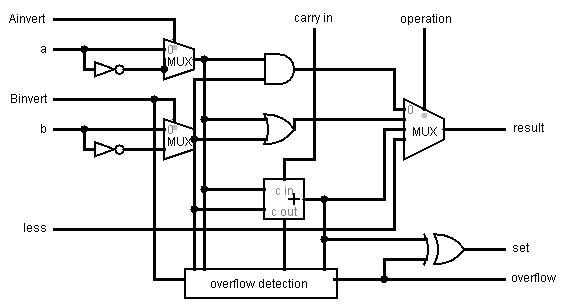
\includegraphics[width=\textwidth]{problem1.png}
    \end{center}
\end{figure}
When overflow has occurred and the highest result bit of the adder is \(0\), this is negative overflow and so we should have set
equal to \(1\). When overflow has occurred and the highest result bit of the adder is \(1\), this is positive overflow and so
we should have set equal to \(0\). Thus doing overflow xor the result of the adder will produce the correct set output.

\section*{Problem 2}

Consider the following truth table for the \(1\)-bit adder of the highest bit.
\[\begin{array}{c|c|c|c|c|c}
        A & B & C_\text{in} & C_\text{out} & \text{Result} & \text{Overflow}\\
        \hline
        0 & 0 & 0 & 0 & 0 & 0\\
        0 & 0 & 1 & 0 & 1 & 1\\
        0 & 1 & 0 & 0 & 1 & 0\\
        0 & 1 & 1 & 1 & 0 & 0\\
        1 & 0 & 0 & 0 & 1 & 0\\
        1 & 0 & 1 & 1 & 0 & 0\\
        1 & 1 & 0 & 1 & 0 & 1\\
        1 & 1 & 1 & 1 & 1 & 0
\end{array}\]
Overflow occurs when both inputs \(A\) and \(B\) are \(0\) and the result is \(1\), which corresponds to
the conditions \(A\geq 0\), \(B\geq 0\), and \(\text{Result}<0\). This is the first row in figure 3.2 in the book.
Overflow also occurs when both inputs \(A\) and \(B\) are \(1\) and the result is \(0\), which corresponds to
the conditions \(A<0\), \(B<0\), and \(\text{Result}\geq 0\). This is the second row in figure 3.2 in the book.
Note that in this truth table, \(C_\text{in}\oplus C_\text{out}\) is \(1\) when overflow occurs and \(0\) otherwise.

Now consider implementing subtraction with this adder. In this case, we simply need to invert the bits of one input and add the
intverted number to the other number, along with a carry in. Because our overflow detection works for addition, this should
also detect overflow in subtraction, as all bits will be flipped on one input. For the flipped numbers, the leading bit of a negative
number will become \(0\) and the leading bit of a positive number will become \(1\). So this also implements the same conditions as the
third and fourth rows in figure 3.2 in the book. So overflow will be properly detected in all cases if we use xor \(C_\text{in}\) and
\(C_\text{out}\) as our overflow signal.

\section*{Problem 3}

Because the \texttt{and}, \texttt{or}, and \texttt{nor} operations do not depend on the output of the adder, their results will be the same.
Additionally, the \texttt{add} operation normally has a carry in of \(0\), so it will not be affected either. However, \texttt{sub}
will always output one below the desired result. In the case that the result is supposed to be the most negative integer, \texttt{sub}
will overflow and output the most positive integer instead. Additionally since \texttt{slt} relies on \texttt{sub}, it will return \(1\) for values that are equal, instead of returning \(0\).

\section*{Problem 4}

\section*{Problem 5}

\section*{Problem 6}

\section*{Problem 7}

\section*{Problem 8}

\end{document}